% Start here


\chapter{Introduction}
\label{sec:intro}

The aim of this document is to report the results of the task T7.1 of WP7:  ``Primary Toolchain Analyses and Recommendations''.

\section{Executive Summary}

The task of WP7 is to produce an integrated chain of software tools that covers according to the approved openETCS FPP all artifacts needed to formalize, modeling, software generation and verification and validation of the entire ETCS System Requirement Specification (Subset 026 and supporting subsets).

To simplify the selection process, this has been separated into a primary and secondary toolchain in the WP7 Description of Work (DoW) \citep{WP7_D01}.  This document is concerned with the selection of methods and tools for the \emph{primary} toolchain, which are means and tools to specify and design a critical system from the system specification to the executable code. Secondary methods and tools selection concerns means to complete the toolchain to obtain a proper engineering environment for the development of critical systems: thus means and tools for verification and  validation activities, to support safety analysis or data or requirement management will be analyzed during this second phase.  As the tools shall be integrated, the selection of an integration platform was required as well.

Eclipse was selected as tool platform, and the decision was unanimous, see Section~\ref{sec:platform}.

Use of SysML and Papyrus for the highest level of specification was also a unanimous decision, see Section~\ref{sec:decision_meeting}. 

Three toolchains have been proposed to complete the use of SysML and Papyrus, which will be referred to with the following shortcuts for brevity:

\begin{description}
\item[SCADE.] This toolchain is based on SCADE in connection with Papyrus, for which an integration already exists.

\item[EFS.] This toolchain is based on ERTMS Formal Specs (EFS), in connection with Papyrus, for which an integration has to be developed.  It will take advantage of elements from the Eclipse ecosystem (and from TOPCASED, wherever possible).  The methods for integrating the various models have to be developed, as well as the gluing code that will hold everything together.

\item[B.] This toolchain is based on B in connection with Papyrus, for which an integration has to be developed.

\end{description}

SCADE is the perfect candidate for a backup plan: While offering pretty much everything the project needs, it has a major drawback: SCADE is not open source.  At the same time, SCADE is a backup that could be activated very quickly.  It is preferable to model successfully with a closed-source solution than to fail with an open one.  But of course, modeling successfully with an open source solution is what we should strive for.

As all three solutions use Papyrus as the first modeling tool, activities should focus on narrowing down which elements of Papyrus should be used.  Once this is clear, WP3 can get started with their modeling activities.

Some effort needs to be spent on defining the interfaces between the various tool elements.  This has been demonstrated nicely by the B-team, as visualized in Figure~\ref{fig:classical-b-toolchain}.  The EFS-team updated their proposal with a similar picture.

The interfaces of the three toolchains should be aligned as much as possible.  Doing so will allow to switch tool components between the three toolchains with comparatively little effort, if the need arises.

Once the toolchains are defined in detail, a pilot model will be created using the B and EFS toolchains.  This pilot will be the foundation for deciding on one single toolchain, by the end of 2013 the latest.

Section~\ref{sec:decision} contains specific decisions intended to concisely guide activities until the end of 2013.

\section{T7.1 Objective}

The goal of WP7 is to provide other openETCS work packages with tooling for their activities.  Tools have been separated into primary and secondary tooling.  Task T7.1 is concerned with the identification of the best primary tooling, considering all constraints of the project.  Selecting tools also entails selecting modeling languages and an integration platform.

 \begin{figure}[b!]
  \centering
  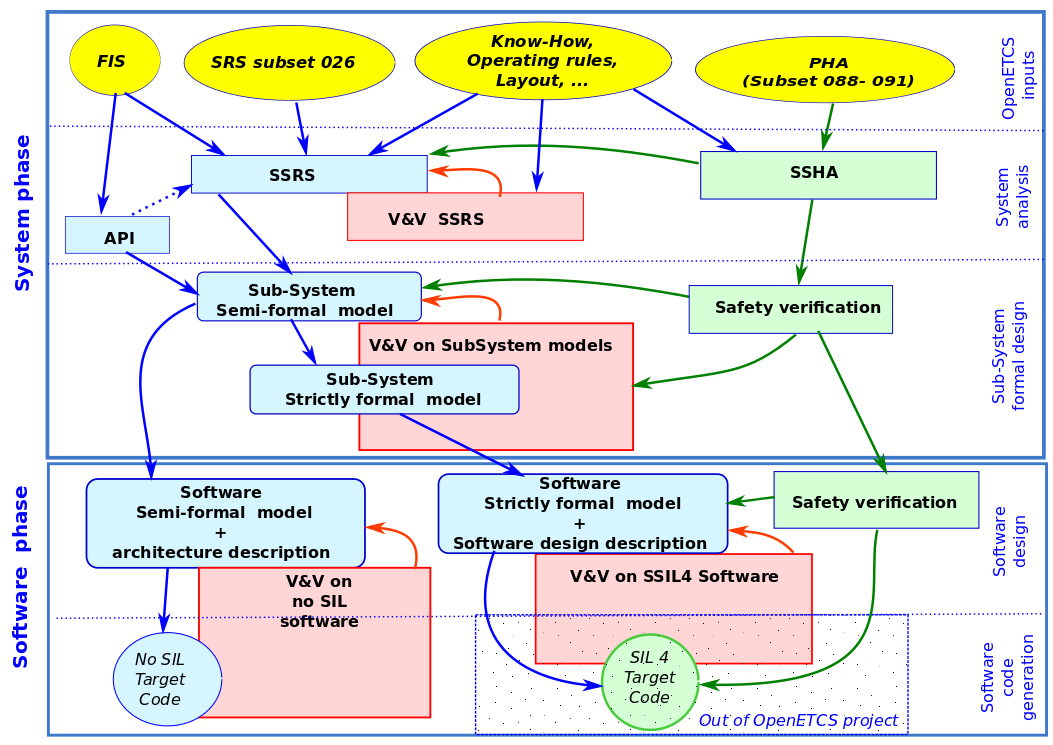
\includegraphics[scale=0.45]{images/WholeProcess.png}
  \caption{Main OpenETCS process.  The models that are covered by primary tooling are shown in blue.}
  \label{fig:main_process}
\end{figure}


\section{Scope of Task T7.1}

The scope of the primary tooling has been defined in the WP7 Description of Work \citep{WP7_D01}.  Figure~\ref{fig:main_process} depicts the main process (taken from \citep{D2_3}, for more details on the process and the meaning of formal methods, please to look at \citep{D2_3} and \citep{D2_4}).  In the scope of the primary tooling are (according to the DoW):

\begin{description}
  \item [Sub-System Semi-formal model.]  ``A semi-formal model of the system specification is defined from the SSRS. This model shall reflect the architecture defined in SSRS. (...) The semi-formal model shall be as consistent as possible with the SSRS level of abstraction, in particular choices concerning
software architecture and design have not to be described at this level. In practice, all the requirements of SSRS and of the sub-system Hazard analysis shall be covered by the semi-formal model.'' (D2.3, 4.4.3). In particular the architecture shall allow "to classify Vital versus Non-Vital items (functions, input/output, requirements, ...) from the
safety analysis results" (D2.3, 4.3.3). "This model shall reflect the
architecture defined in SSRS " (D2.3, 4.4.3).
 ``The means of description of the semi-formal model shall be understandable by domain experts, providing graphical description'' (D2.3, 4.4.4).

  \item [Sub-System Strictly formal model.] ``This semi-formal model \emph{can} be extended with strictly formal models to improve the understanding of some part of the sub-system.'' (D2.3, 4.4.2).  ``To facilitate safety activities, the safety relevant function should be as much as possible insulated from non safety relevant functions.'' (D2.3, 4.4.3).

  \item [Software Semi-formal model + architecture description.] The main output of this step is a semi-formal model which allows to produce executable code. ``This model shall be completed by a Software Architecture and Design Specification, which describes the software architecture and the design choices. (...) The semi-formal model defined during the system phase shall be completed, keeping the same language or extending it to cover specific software aspects.'' (D2.3, 4.5.2).

  \item [Software Strictly formal model + Software design description.]  This model is concerned with the functional and safety branch.  This activity ``shall provide methods and a toolchain to obtain SIL4 executable code of the on-board software application.'' (D2.3, 4.5.3). Inparticular T3 class tools shall be necessary  to  automatically produce SIL4 code form software model.

\end{description}


\subsection{Scope with respect to SSRS, API and code}

API, Code and SSRS\footnote{Note that the DoW does not even mention the SSRS, as its creation has been proposed the first time in February 2013, when the DoW was already finalized.  Therefore, we include SSRS-related activities with T7.2.3 (Requirement traceability) and report on them in O7.2.5 (Requirement management tool choices).}  are in the scope of the secondary toolchain (T7.2).  Choices in the primary toolchain that may affect the secondary toolchain will be covered in this document.

The SSRS poses a special challenge, as activities in its creation have already started.  However, no tools have been selected yet.  Deliverable D2.3 \citep{D2_3} describes the form of the SSRS as follows:
``The SSRS (...) shall be described as textual documents.'' (D2.3, 4.3.4).  It continues to state: ``However these documents shall be completed by a semi-formal model to describe the functional architecture of the on-board unit''.

The connection between SSRS and Sub-System Semi-formal model is described as: ``A semi-formal model of the system specification is defined from the SSRS. (...) In practice, all the requirements of SSRS and of the subsystem Hazard analysis shall be covered by the semi-formal model.''

There is even less information regarding the API, except that it is handled corresponding to the SSRS: ``The SSRS and API shall be described as textual documents. However these documents shall be completed by a semi-formal model to describe the functional architecture of the on-board unit.'' (D2.3, 4.3.4).

There is little relevant information with regard to code generation in this report, except that it makes some implications regarding the software functional model: ``A first executable code is produced from the software functional model.  This executable code shall be non vital. However, it shall be able to run in real time on a on-board computer.  Thus, it shall comply to the standardized interfaces.'' (D2.3, 4.6.2).

\section{Organization of this Report}

This report is organized as follows:

\begin{description}
\item[Introduction (Section \ref{sec:intro}).] An executive summary, as well as an overview of the WP7 Task T7.1 activities.  It shows how T7.1 fits into openETCS in general and WP7 in particular.  It also describes the scope of the results described in this deliverable, making sure the boundary to the secondary toolchain is properly defined.

\item[Results on Means and Tools (Section \ref{sec:results}).] A short description of the three proposed toolchains.  The selection process is described in detail.

\item[Discussion and Results on Tool Platform (Section \ref{sec:platform}).] A description of the proposed tool platform and results of selection is given.

\item[Decision (Section \ref{sec:decision}).] This conclusion sums up  the pro and cons of each proposals and gives the decisions made by the consortium.

\item[Detailed Description of the Toolchains (Appendices).] The detailled description of each toolchain is given in Appendix \ref{sec:sysML-Scade} For SysMl and Scade, \ref{sec:sysML-EFS} for SysML and EFS and \ref{sec:sysML-B} for SysML and B.


\end{description}

%\section{T7.1 activities}

%The activities have started in November 2012, with the completion of the WP7 DoW and consequently the organization of the benchmark.  

%After selection of a set of case studies (specified in D2.5 \citep{D2_5}), different approaches have been proposed and models have been stored on a common open github repository. All the methods have been presented during a public meeting in April 2013.

%Besides, a set of criteria have been defined according the D2.6-9 requirement document \citep{D2_6}.  The results are recorded in the outputs O7.1.3-O7.1.7 \citep{WP7_O713_O717} for means and tools and O7.1.9 \citep{WP7_O719} for tool platform.

%A decision meeting took place the 4th of July 2013 to analyze the results of the benchmark and to decide which means and tools will be retained during the process.

%Results of the decision are given in this current document. 



%%%%%%%%%%%%%%%%%%%%%%%%%%%%%%%%%%%%%%%%%%%%%%%%%%%%%%%%%%%%%%%

\section{Glossary}
\label{sec:glossary}

\begin{description}
\item[API] Application Programming Interface
\item[DoW] Description of Work.  In this document we typically mean the WP7 DoW.
\item[DSL] Domain Specific Language
\item[EMF] Eclipse Modeling Framework
\item[FIS] Functional Interface Specification
\item[HW] Hardware
\item[I/O] Input/Output
\item[OBU] On-Board Unit
\item[PHA] Preliminary Hazard Analysis
\item[SIL] Safety Integrity Level
\item[SSIL] Software Safety Integrity Level
\item[SRS] System Requirement Specification
\item[SSHA] Sub-System Hazard Analysis
\item[SSRS] Sub-System Requirement Specification
\item[SW] Software
\item[SWOT] Strengths, Weaknesses, Opportunities, Threats
\item[V\&V] Verification \& Validation
\end{description}

%%%%%%%%%%%%%%%%%%%%%%%%%%%%%%%%%%%%%%%%%%%%%%%%%%%%%%%%%%%%%%%


